\chapter{Foundations}
\label{ch:Foundations}

Maintaining consistency among multiple models of a single system requires a technical foundation for representing those models.
It also requires a mechanism that detects changes in the models and a language that defines the necessary repair actions.
The \hyperref[sec:Foundations:EMF]{Eclipse Modeling Framework} covers the first aspect by defining how metamodels, models and their modifications are represented.
\hyperref[sec:Foundations:Vitruvius]{Vitruvius} builds on this foundation by combining independent models into a Virtual Single Underlying Model (V-SUM).
Consistency is restored within the V-SUM by rules written in the \hyperref[sec:Foundations:ReactionsLanguage]{Reactions Language} \cite{KLARE2021110815}.
Java source code is included through \hyperref[sec:Foundations:JaMoPP]{JaMoPP}, which represents it as an ordinary model and thereby subjects it to the same mechanism \cite{heidenreich2009closing}.
To introduce variability, the system is viewed as a \hyperref[sec:Foundations:SoftwareProductLines]{Software Product Line}.
Features, feature models, and configurations describe the variability of a common set of assets \cite{clements2002software,kang1990feature}.

\section{EMF}
\label{sec:Foundations:EMF}

The Eclipse Modeling Framework (EMF) is as a modeling framework and code generation facility designed for developing tools and applications that utilize a structured data model \cite{emf}.
It implements the Essential Meta-Object Facility (EMOF) metamodel, which defines the standard core modeling concepts necessary for model creation \cite{omgMof}.
EMF realizes the EMOF metamodel through Ecore, which serves as its technical implementation.
Ecore provides classes for defining models, attributes, references, operations, and is capable of generating change events \cite{emfDocs}.

Model levels represent distinct abstractions of a real-world system.
In \autoref{fig:emf-levels}, the connections between them are shown \cite{bezivin2005bridging}.

\begin{figure}[htbp]
    \centering
    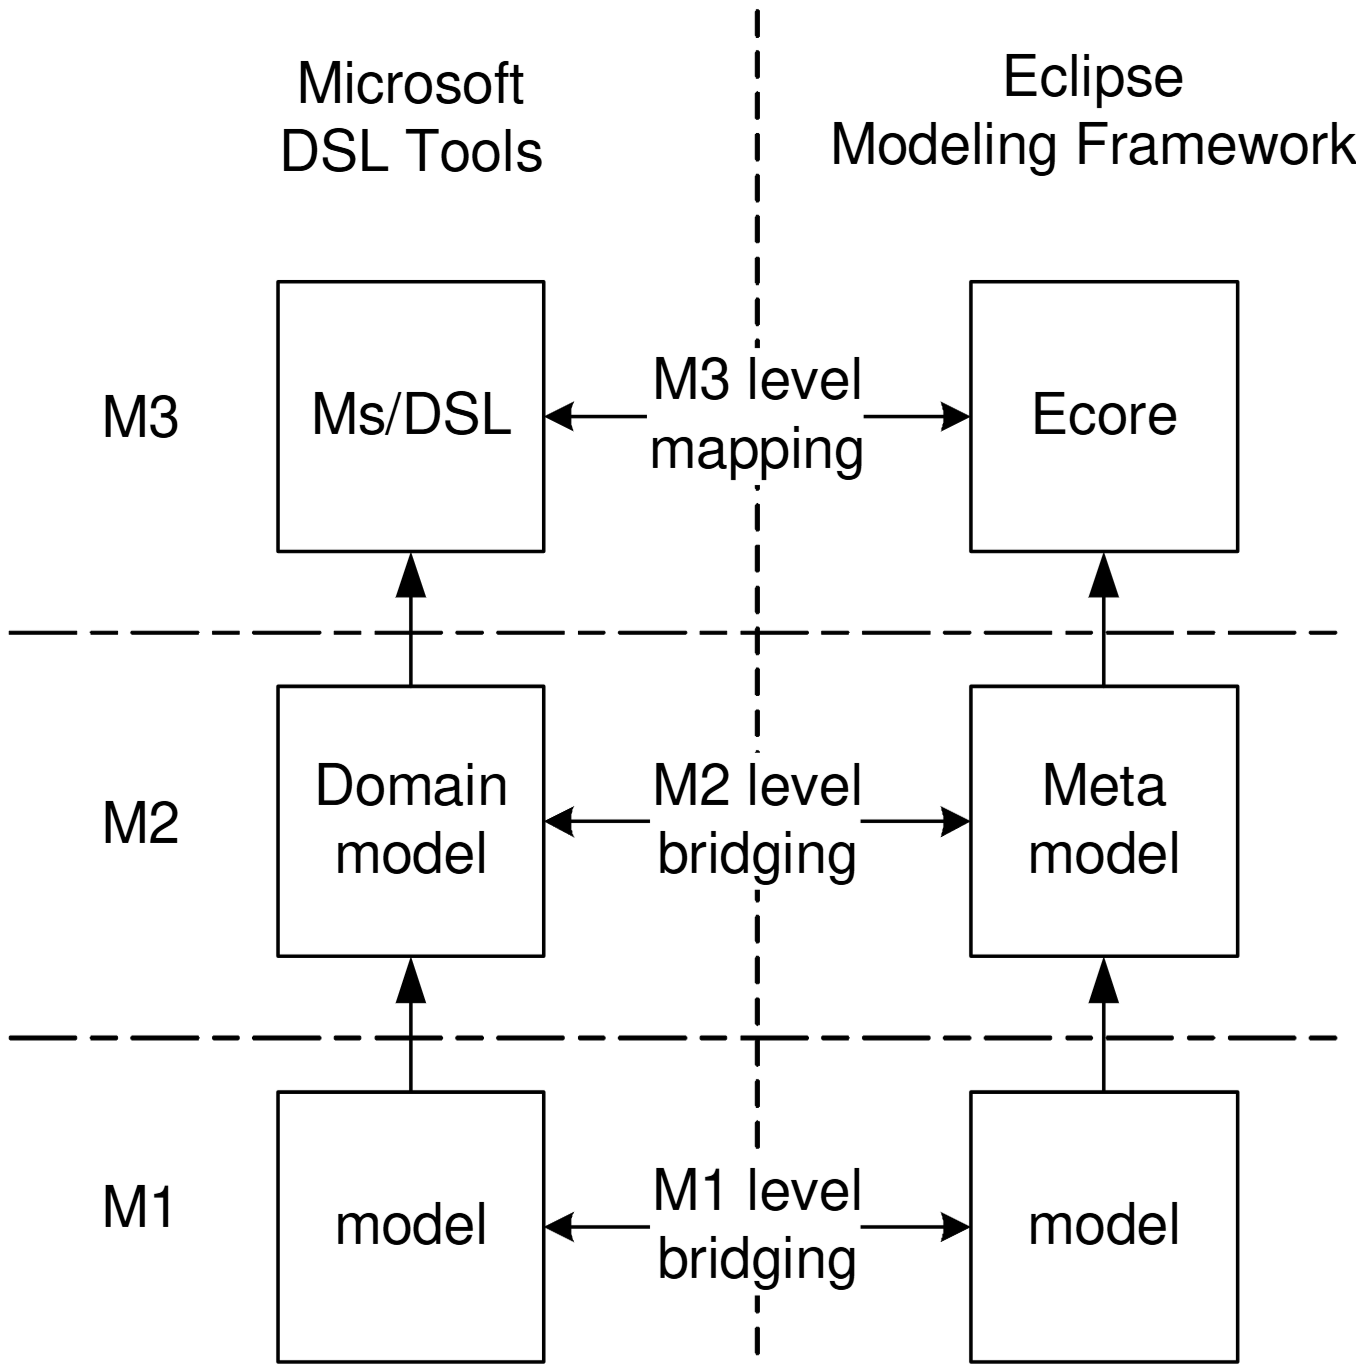
\includegraphics[width=.6\linewidth]{figures/emf-levels.png}
    \caption{Connection between model levels \cite{bezivin2005bridging}}
    \label{fig:emf-levels}
\end{figure}

M0 is not visible in \autoref{fig:emf-levels}.
This represents a real system without any kind of abstractions.
M1 is used for the first layer of abstraction representing models.
These models represent instances close to existing elements, such as Java code.
One level further, metamodels are defined.
A metamodel represents the world in which models live.
It provides a comprehensive definition of metaclasses.
It is evident that each element of a model on M1 is an instance of precisely one of them \cite{kuhne2006matters}.
Both UML and JaMoPP are examples of metamodels.
Consequently, a class in Java source code is therefore an instance of a metaclass defined by JaMoPP.
This principal finds equal application in the context of a class within a UML model, which constitutes an instance of a metaclass defined by UML \cite{heidenreich2009closing,bezivin2005bridging}.
The final level, M3, is referred to as the meta-metamodel.
This level defines the conceptual framework that is applicable for the definition of metamodels \cite{omgMof}.
In the context of EMF, Ecore assumes responsibility for this process.
It provides constructs such as \texttt{EClass}, \texttt{EAttribute}, and \texttt{EReference}, through which metamodels like UML or JaMoPP are expressed.
The presence of a meta-metamodel, defined in terms of itself, prevents the existence of any additional level of abstraction.
The Ecore model is the basis for the description of Ecore, thereby establishing that \texttt{EClass} is an instance of \texttt{EClass}.
An additional level would only repeat the concepts already present on M3 and is therefore omitted \cite{emfDocs,omgMof}.

Ecore facilitates the utilization of metamodels in the work.
It is possible to group each metamodel by its namespace URI with an \texttt{EPackage} stored in a global package registry.
\texttt{EClass} represents a metaclass capable of holding different structural features, like \texttt{EAttribute} or \texttt{EReference}.
The reference can be classified as either containment or non-containment.
It is shown that each object is limited to at most one \texttt{eContainer}, allowing the model to form a containment tree.
Roots have no container and sit directly in a resource.
The deletion of an object from its container also results in the removal of the subtree and the reference that points to it \cite{emfDocs}.

A notification is dispatched for each modification.
It carries the event type, the structural feature as well as both the old and new values.
The responsibility for receiving these notifications falls upon an \texttt{EContentAdapter} \cite{emfDocs}.

The persistence of models is an inherent feature of EMF.
A \texttt{Resource} represents a unit of persistence.
Addressing it works with URIs, and it gets saved and loaded as a whole.
The working context, which is responsible for loading resources and resolving references between them, is referred to as a \texttt{ResourceSet}.
A reference to an element in another resource is stored as a URI that identifies the target resource, together with a fragment identifying the element within it.
The ResourceSet resolves such a reference in a lazy manner, which means that the target resource is loaded only once the reference is accessed.
The process of resolution facilitates the conversion of a potentially logical URI into a physical one, thereby enabling the factory registry to select the parser for that particular resource.
\texttt{XMI} would be used for \texttt{.uml} files, while \texttt{JaMoPP} is utilized for \texttt{.java} files \cite{emfDocs,heidenreich2009closing}.
XMI is utilized for the purpose of serialization within the EMF framework.
In this approach, each resource is allocated to its own file.
It is important to note that the references contained within are URI fragments.
By default, these are positional paths depending on the order, but they can also be fixed \texttt{xmi:ids} \cite{omgXmi,emfDocs}.

\section{Vitruvius}
\label{sec:Foundations:Vitruvius}

One of the most important foundations for this thesis is Vitruvius itself.
Vitruvius is a framework for managing and keeping models consistent in a model-driven engineering context.
In a typical MDE system, different domain experts work with their own models, each describing a particular aspect of the same system.
Because all of these models describe different aspects of the same reality, they have overlapping information and must stay consistent with each other \cite{KLARE2021110815}.

One possible solution for keeping multiple models consistent is the view-based approach.
In theory, a Single Underlying Model (SUM) would contain all information about the system, and different views would simply project the relevant subset to each expert.
Often it is not feasible to have such a single monolithic model representing all aspects of a system, so Vitruvius introduces the concept of a V-SUM \cite{amrani2024survey,hermann2024towards}.
A V-SUM combines multiple independent models and exposes views to interact with them, giving the illusion of a single source of truth.
The process surrounding a V-SUM defines two distinct roles.
The methodologist is tasked with the creation of the V-SUM metamodel, a process that involves the selection of the involved metamodels, the establishment of the consistency preservation between them, and defining view types.
Consequently, the focus is on metamodel elements.
The developer utilizes the predefined views to create, access, and manipulate the V-SUM, without having the capability to modify the V-SUM metamodel itself \cite{KLARE2021110815}.

The consistency preservation mechanism in Vitruvius is based on Consistency Preservation Rules (CPRs).
A CPR specifies the requisite response to a particular change in a single model to restore consistency with related models.
The CPRs are specified using the Reactions Language, which provides the methodologist with a structured means of expressing these rules without resorting to general-purpose code \cite{KLARE2021110815}.
Reactions generate a set of \texttt{ChangePropagationSpecifications}, which are then employed to construct a V-SUM.
The remaining components necessary for the construction of a V-SUM include the metamodels themselves, a user interactor and a designated storage folder, where all data will be stored \cite{vitruviusGithub}.
One thing getting persisted are correspondences.
They function as an identifying link between elements from various models.
Reactions establish explicit correspondences and can be used to record which element was derived from which \cite{KLARE2021110815}.

Building upon the foundations laid out in \autoref{sec:Foundations:EMF}, atomic changes can be created by implementing an EContentAdapter to receive notifications.
Upon receiving a notification an atomic change is initiated, documenting a specific modification, such as the creation, deletion, insertion, removal or replacement of an element.
Changes are ordered within a \texttt{transactional change} \cite{KLARE2021110815}.

A view is defined as a copy of models in its own ResourceSet and edits are confined to the view's ResourceSet.
The two methods of capturing edits depend on its trait.
The conventional delta-based approach is employed for the purpose of recording change, whereby each EMF notification is transformed into an atomic change.
An alternative approach is to adopt a state-based model.
Upon the commit of a view, a comparison is started between its previous and current states, thereby deriving any alterations that occurred.
A commit transmits changes to the V-SUM itself, where they are implemented in its own models and subsequently transferred to specifications.
Those alter target models and correspondences, thereby introducing new changes \cite{KLARE2021110815,wittler2023evaluating}.

Even though Vitruvius' consistency preservation system typically operates automatically, there are some circumstances where manual intervention is still required.
An interactive dialog can be used to prompt the user when a reaction does not have enough information to determine how to proceed.
The user can choose between several options, accept or reject a transformation, or even enter custom data.
For instance, the framework may not be able to determine whether a new class in the source code represents a basic utility class or an architectural component.
In these situations, a dialog prompts the developer for clarification before carrying out the transformation \cite{vitruviusGithub}.
Although this mechanism increases flexibility, it also introduces runtime variability because the result is contingent upon the user.

\section{Reactions Language}
\label{sec:Foundations:ReactionsLanguage}

The Reactions language is an imperative DSL designed to work with provided delta events to keep models consistent.
It has two basic building blocks: Reactions and Routines.
Reactions are triggered through change events and will call the corresponding routines to perform the necessary repair actions on other models \cite{KLARE2021110815}.
Routines contain the actual logic to update the models.
They can call other routines or directly manipulate the models to achieve consistency.
A routine has three phases, which are \textit{match}, \textit{create} and \textit{update}.
In the match phase preconditions are checked to see if this routine is applicable for the given change and required resources are acquired.
One precondition is the check guard, which can test any arbitrary condition.
If the match phase is successful, the create phase will generate any new elements needed for the update.
Finally, the update phase will perform the actual routine calls and model manipulations to restore consistency in this model \cite{reactionsDocumentation}.
The language is implemented using Ecore and Xtext, which is a framework for developing DSLs in Eclipse.
The actual code can be written in Xtend, a statically typed programming language that compiles to Java source code, but offers some additional features to make the code more concise \cite{xtext,xtend}.
It is important to note that each Reaction has already been assigned a qualified name \cite{reactionsDocumentation}.
This is necessary for subsequent developments.

\section{JaMoPP}
\label{sec:Foundations:JaMoPP}

The Java Model Parser and Printer (JaMoPP) is an Ecore metamodel for Java as well as a parser and a printer.
The parsing of a given URI inside EMF is managed by the resource factory registered for the specific type.
JaMoPP has been identified as the primary resource factory for the \texttt{.java} domain.
The source code can be parsed into a model, and subsequently "printed" back as code.
This is a requisite, given that with the context of Java, source code assumes the role of the model file.
It is important to note that every element is regarded a compilation unit, including individual expressions.
In contrast to EMF, references are not stored as URIs.
These issues are resolved by a qualified name against a global classpath registry, which is not part of a single V-SUM.
A significant distinction between EMF and Java is the inability of Java elements to carry identifiers directly, as the source code lacks the capability to store them \cite{heidenreich2009closing}.

\section{Software Product Lines}
\label{sec:Foundations:SoftwareProductLines}

Software Product Lines (SPL) represent an evolution of traditional product lines into the digital domain.
SPL's area of expertise lies in the field of software artifacts, as opposed to physical products.
Those artifacts are derived from a shared set of software assets.
This facilitates the development of multiple software products that share common features, while still allowing for variability and customization \cite{clements2002software,bachmann2005variability}.
It happens in two distinct phases.
Domain engineering is concerned with the creation of assets and the variability, while application engineering is concerned with the derivation from these assets \cite{pohl2005software,apel2013software}.
In this thesis, the assets are the annotated reactions, which collectively form a 150\% model.
A configuration is defined as the set of selected features, and the product is the rule set derived from it, which reduces the 150\% model to a 100\% model \cite{kaestner2008granularity,czarnecki2005mapping}.

A feature is defined as a unit of variability, that serves to distinguish products from each other.
The generation of a configuration from a comprehensive array of features requires a set of guidelines on how to combine them.
It is evident that a feature model fulfils this purpose, by creating restrictions on combinations of different features.
The features contained within can be modelled as a tree with different group types.
\texttt{Mandatory} requires that every feature in the group be selected if the parent feature is selected.
The utilization of an optional group facilitates the selection of children, although this is not required.
For an \texttt{alternative}, it is necessary that exactly one of the children is selected, thereby representing an XOR relation \cite{van2001notion,kang1990feature}.
The ability to select at least one child is modelled by \texttt{or}.
Cross-tree constraints represent dependencies that cannot be modelled in any other way \cite{nevsic2019principles}.
The creation of a textual representation of a feature model is possible in \texttt{uvl}, which is the result of a community effort to establish a unified language for variability models \cite{uvl}.

A configuration that is deemed valid is one that satisfies the group types and all cross-tree constraints.
Validity may be regarded as a satisfiability check, a function performed by tools like Flamapy IDE \cite{white2010automated,flamapy-ide,kastner2009featureide}.